\documentclass{article}
\usepackage{iclr2026_conference,times}

\input{math_commands.tex}

\usepackage{amsmath,amssymb,amsthm}
\usepackage{booktabs}
\usepackage{graphicx}
\usepackage{microtype}
\usepackage{url}
\usepackage{hyperref}

\newtheorem{theorem}{Theorem}
\newtheorem{proposition}{Proposition}

\title{Exact Test-Time Inference Laws for Best-of-N World-Action Rollout Selection}

\author{Anonymous Authors}

%\iclrfinalcopy
\begin{document}
\maketitle

\begin{abstract}
Embodied planners increasingly sample candidate futures, score them with a planner or verifier, and execute the highest-scoring rollout. We study the fixed-generator, fixed-scorer inference question: how much real utility should best-of-$N$ rollout selection buy? For finite empirical rollout pools, we prove an exact tie-aware law for expected selected real utility under i.i.d. with-replacement sampling, max-score selection, and uniform maximum-score tie-breaking. The law shows that the value of larger $N$ is governed by real utility in the upper planner-score tail; aligned tails yield gains, exhausted tails saturate, and misaligned tails can reduce real utility. Binary success is a special case, yielding an exact $N=2$ tie-aware AUC identity, while $N>2$ depends on higher upper-tail rank moments beyond AUC. Experiments check the law and illustrate alignment, mismatch, falsification, learned WAM-lite, adaptive-budgeting, and simulated rollout-pool regimes. The paper is not a WAM training scaling law, not real-world robot validation, not modern VLA-scale validation, not full RoboCasa-wide validation, and not a universal OOD/generalization guarantee.
\end{abstract}

\section{Introduction}

Modern embodied agents increasingly act by imagining candidate futures. A learned world model or generative policy proposes rollouts; a planner, verifier, value model, reward model, or hand-designed heuristic scores them; the planner executes the highest-scoring rollout, or the first action of it. Related verifier and best-of-$N$ alignment work studies the same sample-many/rerank primitive \citep{cobbe2021verifiers,beirami2024bestofn}. This pattern appears in latent world-model planning \citep{ha2018worldmodels,hafner2019planet,hafner2020dreamer}, model-based reinforcement learning and sampling MPC \citep{chua2018pets,rubinstein1999cem,williams2017itmmpc}, and the broader move toward generative robot policies and vision-language-action systems \citep{brohan2022rt1,brohan2023rt2,chi2023diffusionpolicy,octo2024}.

This makes test-time rollout sampling a basic inference knob. If a planner or simulated agent can sample 1, 8, 32, or 128 candidate futures before acting, how many should it sample? The usual answer is operational rather than conceptual: sample more when compute allows. But best-of-$N$ selection is not automatically beneficial. Sampling more candidates selects deeper into the planner-score tail. If that tail contains truly high-utility rollouts, extra imagination helps. If that tail contains rollouts that only look good under the model or scorer, extra imagination can saturate or even reduce real utility.

This paper isolates the inference question from the training question. For a fixed generator and scorer, finite empirical rollout pool, i.i.d. with-replacement sampling, max-score selection, and uniform maximum-score tie-breaking, the answer is exact: best-of-$N$ performance is determined by the joint distribution of planner score and real rollout utility. The relevant object is not average prediction accuracy alone. It is the real utility of rollouts in the upper planner-score tail.

The binary setting exposes a sharp boundary for familiar ranking summaries. For $N=2$, selected success is determined by the success rate and a tie-aware AUC term. For $N>2$, AUC alone is insufficient: larger candidate pools depend on higher upper-tail rank moments. Thus the same two-sample ranking quality can lead to different high-$N$ rollout-selection value.

We check this picture with artifact-backed experiments. Controlled analytic cases test the exact law, the AUC identity, and same-AUC/high-$N$ counterexamples. Learned WAM-lite and simulated rollout-pool artifacts illustrate useful, saturated, and harmful regimes. We also use the resulting inference-value profile as a fixed-stack adaptive budgeting heuristic: estimate whether another rollout is likely to buy real utility before spending the sample.

The scope is deliberately narrow. We do not propose a universal world-action-model training law, a Robot Chinchilla-style training rule, a real-world robot result, a modern VLA-scale validation, a full RoboCasa-wide validation, or a universal OOD/generalization guarantee. Instead, we ask:
\begin{quote}
\emph{For a fixed rollout generator and fixed scorer, what is the expected real utility of executing the highest-scoring rollout among $N$ imagined candidates?}
\end{quote}

\paragraph{Contributions.}
First, we prove an exact finite empirical, tie-aware law for best-of-$N$ rollout selection under a fixed generator/scorer, finite empirical pool, i.i.d. with-replacement sampling, max-score selection, and uniform maximum-score tie-breaking. It covers real-valued utility, binary success, and score ties. Second, we give the continuous no-tie population form, the binary success special case, and the exact $N=2$ tie-aware AUC identity. Third, we show why AUC alone is insufficient for $N>2$: larger candidate pools depend on higher upper-tail rank moments. Fourth, we turn the law into an inference-value profile for improvement, saturation, harm, and adaptive rollout budgeting. Fifth, experiments check the laws and illustrate the mechanisms in analytic, learned WAM-lite, and simulated robotics rollout-pool artifacts.

\begin{figure}[t]
\centering
\begin{minipage}{0.49\linewidth}
  \centering
  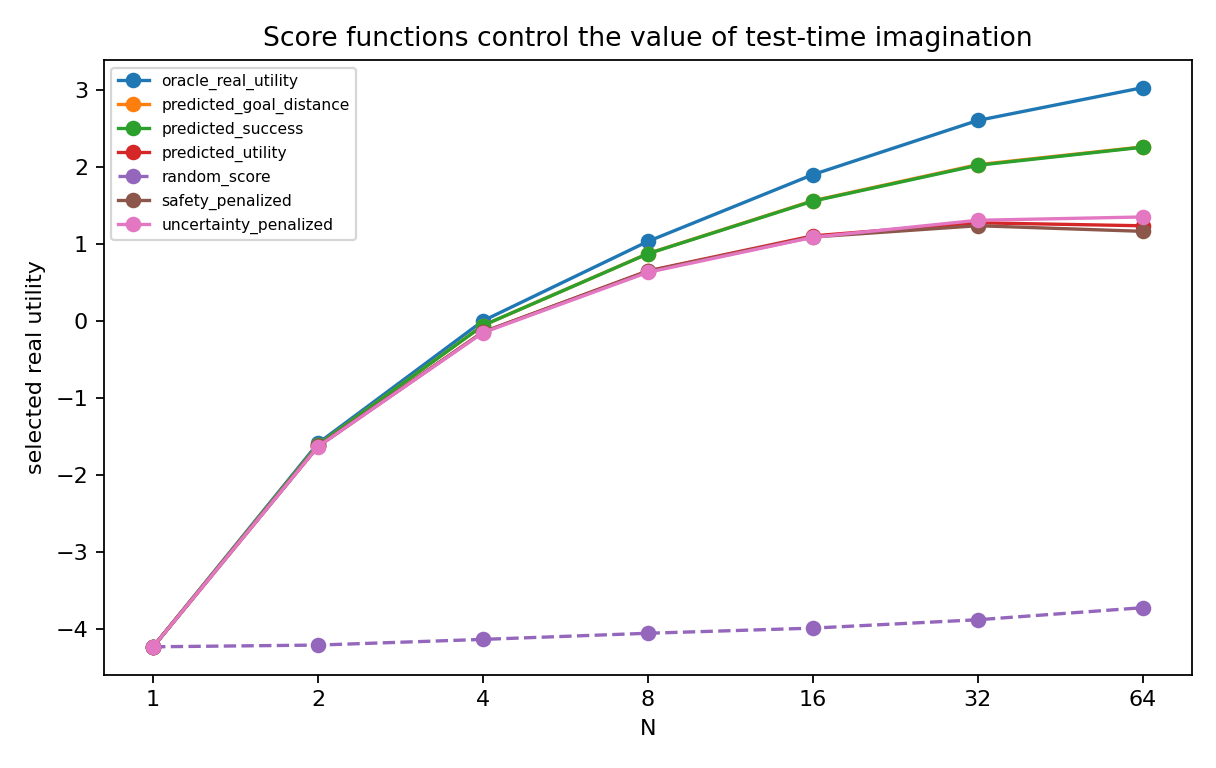
\includegraphics[width=\linewidth]{paper_figures/fig_score_regimes_learned.png}
\end{minipage}
\hfill
\begin{minipage}{0.49\linewidth}
  \centering
  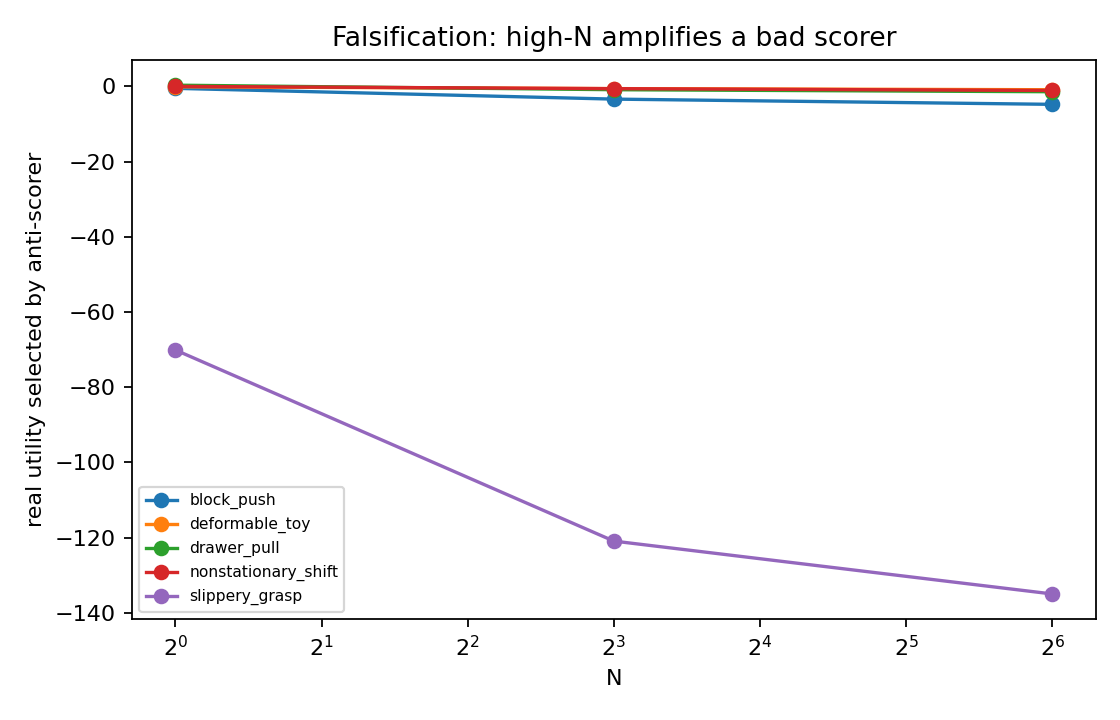
\includegraphics[width=\linewidth]{paper_figures/fig_bad_scorer.png}
\end{minipage}
\caption{\textbf{The value of imagination is a score-tail phenomenon.} Left: aligned learned and oracle-like scores improve selected real utility as $N$ grows, while a random score remains poor. Right: a deliberately anti-aligned scorer can make high-$N$ selection worse. The theorem explains both curves with the same object: the joint distribution of planner score and real utility in the upper score tail.}
\label{fig:regimes}
\end{figure}

\section{Problem Setup}
\label{sec:setup}

Fix a planning state $x$. A rollout generator samples candidate action/future rollouts $Z$. Each sampled rollout has a planner score $S=s(Z)$ used for selection and a real utility $R=r_{\mathrm{real}}(Z)$ measured under the true environment or heldout simulator. In binary tasks, $R=Y\in\{0,1\}$.

Best-of-$N$ world-action planning samples $N$ rollouts independently from the fixed rollout distribution, selects a maximum-score sampled rollout, and breaks maximum-score ties uniformly at random. The inference value is
\[
V_N(x)=\mathbb{E}[\text{real utility of the selected rollout}\mid x].
\]
For binary success, we write $f_N(x)=V_N(x)$.

The fixed-$x$ formulation is intentional. In a receding-horizon controller, the law applies conditionally at each visited state. It does not imply a global closed-form law for arbitrary closed-loop dynamics. Likewise, the theorem assumes that the relevant score/utility distribution or empirical pool is known; estimating it from pilot rollouts is a separate statistical problem.

\section{Exact Finite Inference Law}
\label{sec:finite-law}

The core result is the finite empirical law. This is the form used for tied empirical rollout pools in our experiments.

\begin{theorem}[Finite tie-aware best-of-$N$ law]
\label{thm:finite}
Fix a planning state $x$ and a finite empirical rollout pool $\mathcal{D}_x=\{(S_i,R_i)\}_{i=1}^m$. Sample $N$ rollouts independently and uniformly with replacement from $\mathcal{D}_x$. Select a maximum-score sampled rollout, breaking maximum-score ties uniformly at random. Sort the pool by score in ascending order and group equal-score ties. Tie group $g$ occupies one-indexed ranks $[r_{\min,g},r_{\max,g}]$ and has mean real utility $\bar R_g$. Then
\[
V_N(x)=
\sum_g \bar R_g
\left[
\left(\frac{r_{\max,g}}{m}\right)^N
-
\left(\frac{r_{\min,g}-1}{m}\right)^N
\right].
\]
\end{theorem}

\paragraph{Interpretation.}
The bracketed term is the probability that the maximum score among the $N$ samples lands in tie group $g$. The expected selected utility is therefore a weighted average of tie-group real utilities, where higher score groups receive increasing mass as $N$ grows. This is why best-of-$N$ is governed by the upper score tail.

\paragraph{Binary success.}
For $R=Y\in\{0,1\}$, the same theorem gives the selected success probability $f_N(x)$. Binary success is a special case of the utility-valued law, not a separate mechanism.

\paragraph{Population no-tie form.}
If scores are continuous and ties occur with probability zero, then
\begin{equation}
\label{eq:continuous-utility}
V_N(x)=N\,\mathbb{E}\!\left[R F_S(S)^{N-1}\mid x\right],
\end{equation}
where $F_S$ is the score CDF at state $x$. For binary success with prevalence $p=\Pr(Y=1)$, successful score $S_+\sim S\mid Y=1$, and marginal score CDF $F_{\mathrm{mix}}$,
\begin{equation}
\label{eq:binary-pop}
f_N(x)=Np\,\mathbb{E}\!\left[F_{\mathrm{mix}}(S_+)^{N-1}\mid x\right].
\end{equation}
Equations~\ref{eq:continuous-utility} and~\ref{eq:binary-pop} are useful population intuitions. The finite theorem remains the correct empirical law when scores tie.

\section{AUC for Two Samples, Tail Moments for Many}
\label{sec:auc}

The binary law connects cleanly to AUC only at $N=2$, using the standard tie-aware ranking interpretation of ROC AUC \citep{hanley1982roc}.

\begin{proposition}[$N=2$ tie-aware AUC identity]
\label{prop:auc}
Let $p=\Pr(Y=1)$, let $S_+$ and $S_-$ denote scores conditioned on success and failure, and define tie-aware AUC
\[
\kappa=\Pr(S_+>S_-)+\frac{1}{2}\Pr(S_+=S_-).
\]
Then
\[
f_2=p^2+2p(1-p)\kappa.
\]
\end{proposition}

\paragraph{Interpretation.}
With two samples, success is guaranteed when both sampled candidates succeed; when exactly one succeeds, the planner succeeds exactly when the successful candidate wins the score comparison, with half credit for ties.

For $N>2$, AUC is not enough. Define the successful rollout's marginal score rank
\[
U=F_{\mathrm{mix}}(S_+).
\]
Equation~\ref{eq:binary-pop} becomes
\[
f_N=Np\,\mathbb{E}[U^{N-1}].
\]
AUC fixes the first rank moment needed for $N=2$, but larger $N$ depends on higher powers of $U$. These higher moments emphasize the upper score tail. Two scorers can therefore have the same $p$ and the same tie-aware AUC while producing very different high-$N$ value.

\begin{figure}[t]
\centering
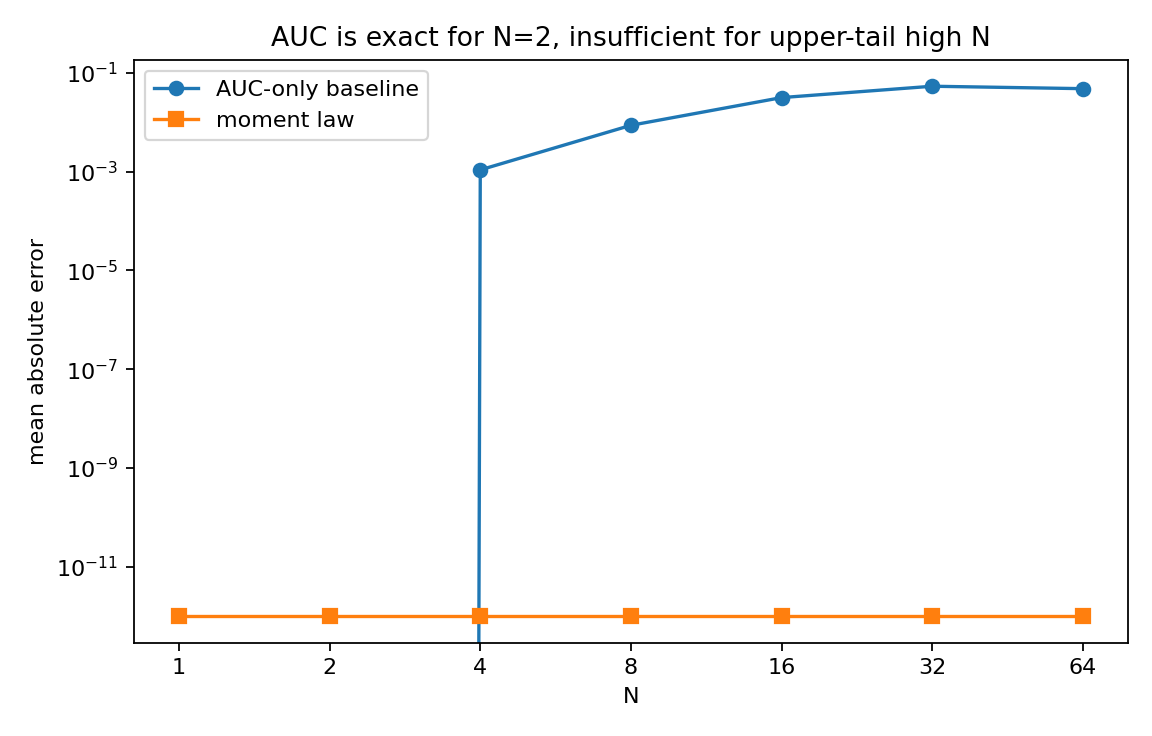
\includegraphics[width=0.70\linewidth]{paper_figures/fig_auc_moments.png}
\caption{\textbf{AUC is exact for $N=2$ and insufficient for high $N$.} AUC-only extrapolation matches the two-sample identity but misses upper-tail behavior as $N$ grows. The moment law tracks the full $N$ curve because it uses $\mathbb{E}[U^{N-1}]$.}
\label{fig:auc}
\end{figure}

\section{Inference-Value Profiles: Improvement, Saturation, and Harm}
\label{sec:profiles}

The theorem turns $N\mapsto V_N(x)$ into an \emph{inference-value profile} for a fixed planning state, generator, scorer, and real utility distribution. The profile is a score-tail accounting object. If high-score rollouts also have high real utility, the curve improves with more samples. If the useful high-score tail is exhausted, the curve saturates. If high-score rollouts have low real utility, the curve can decline.

This view separates score optimization from deployment value. World-action planning is useful because imagined futures can expose good actions before acting. It is risky because the planner selects by score, not by real utility. This echoes model-bias and model-exploitation concerns in model-based reinforcement learning \citep{janner2019mbpo}. If a score aligns with imagined utility but the high-score tail is misaligned with real outcomes, increasing $N$ over-selects rollouts that look good under the model while failing under the environment.

The theorem does not fail in this setting. It predicts selected real utility from the joint distribution of score and real utility. The failure is score/utility alignment. This gives score-tail accounting for how high-$N$ selection can amplify mismatch in tested settings.

\begin{figure}[t]
\centering
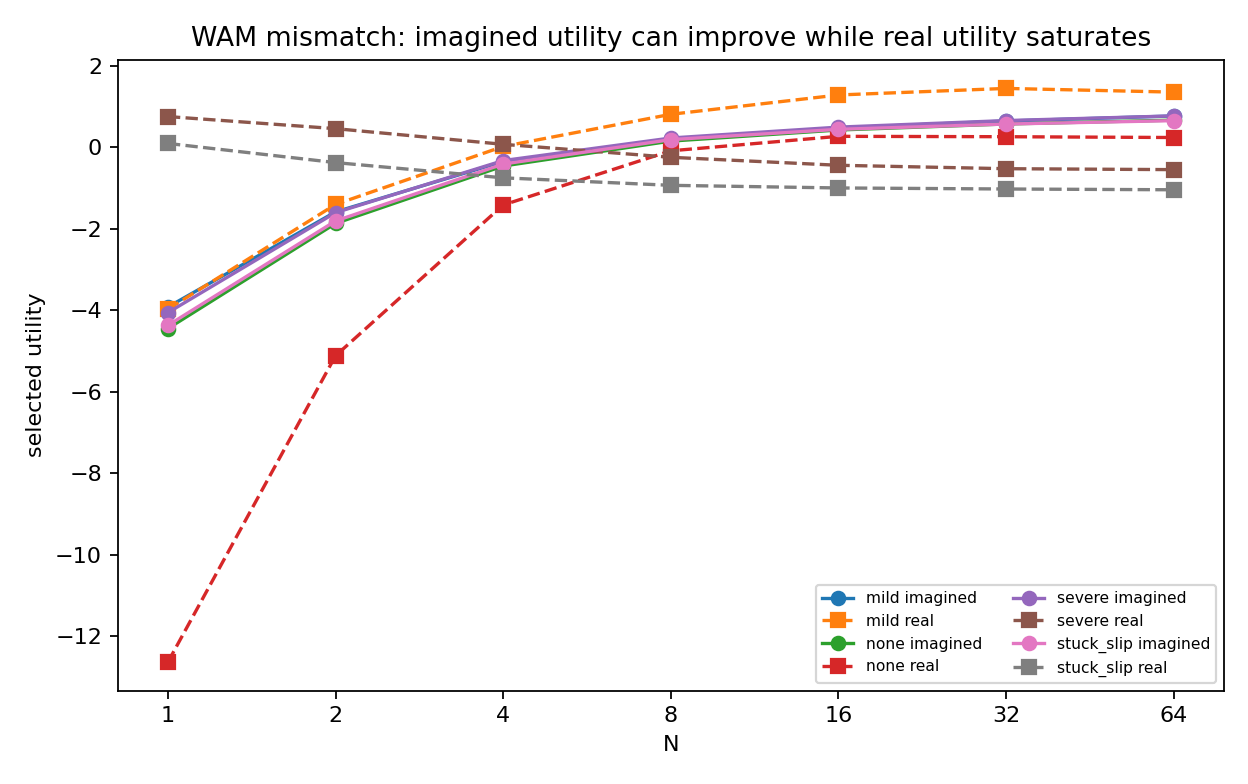
\includegraphics[width=0.74\linewidth]{paper_figures/fig_mismatch.png}
\caption{\textbf{Imagined-real mismatch can hide behind improving model scores.} As $N$ increases, selected imagined utility can improve while selected real utility saturates or degrades. The law says to audit real utility in the high-score tail, not just imagined value.}
\label{fig:mismatch}
\end{figure}

\section{Experiments}
\label{sec:experiments}

Each experiment family checks a theorem claim or illustrates a conceptual consequence.

\paragraph{Exact law and AUC identity.}
Finite empirical checks compare the tie-aware law with Monte Carlo selection. The claim ledger reports binary success MAE $0.00210$, utility MAE $0.01376$, and $N=2$ AUC identity max error $0.0$ in core checks. These tests check the implementation of Theorem~\ref{thm:finite} and Proposition~\ref{prop:auc}.

\paragraph{AUC versus upper-tail moments.}
Controlled same-$p$, same-$\kappa$ examples show that AUC-only summaries can miss high-$N$ behavior. The moment-law predictor remains accurate because it uses the higher rank moments in $f_N=Np\,\mathbb{E}[U^{N-1}]$ (Figure~\ref{fig:auc}).

\paragraph{Score alignment regimes.}
Scorer comparisons include random, learned, heuristic, oracle, safety-penalized, uncertainty-penalized, and deliberately bad scorers. Figure~\ref{fig:regimes} shows both aligned and anti-aligned behavior. The empirical pattern matches the theorem: useful imagination requires real utility in the upper score tail.

\paragraph{Bad scorer and imagined-real mismatch.}
Falsification tests use anti-aligned scorers and compare selected imagined utility with selected real utility (Figure~\ref{fig:mismatch}). These checks illustrate the risk that high-$N$ selection concentrates probability mass on low-real-utility rollouts in the high planner-score tail.

\paragraph{Learned WAM-lite checks.}
Learned WAM-lite artifacts check whether the same inference-value accounting appears beyond analytic score functions. These experiments report learned model errors, exact-law agreement on heldout rollout pools, and learned-scorer versus random-scorer comparisons. They are lightweight learned-model checks, not evidence for a universal WAM training recipe.

\paragraph{Simulated robotics rollout pools.}
We also evaluate in learned WAM-lite and simulator/benchmark rollout-pool artifacts. Verified exact-law MAEs include Gymnasium Robotics Fetch $0.0126$, Gymnasium Robotics RGB visual WAM $0.0106$, ManiSkill state-mode $0.00345$, Meta-World $0.0298$, RoboSuite $0.00237$, RoboCasa 12-task family $0.000292$, RoboCasa residual 35-task clean/cook $0.000246$, and LIBERO rollout-pool WAM-lite $0.000140$. Learned scorers beat random with positive confidence intervals in several rollout-pool benchmarks, including Fetch, Meta-World, RoboSuite, RoboCasa families, and LIBERO rollout-pool checks. These are simulated rollout-pool results, not hardware evidence and not full modern VLA policy validation.

\begin{figure}[t]
\centering
\begin{minipage}{0.49\linewidth}
  \centering
  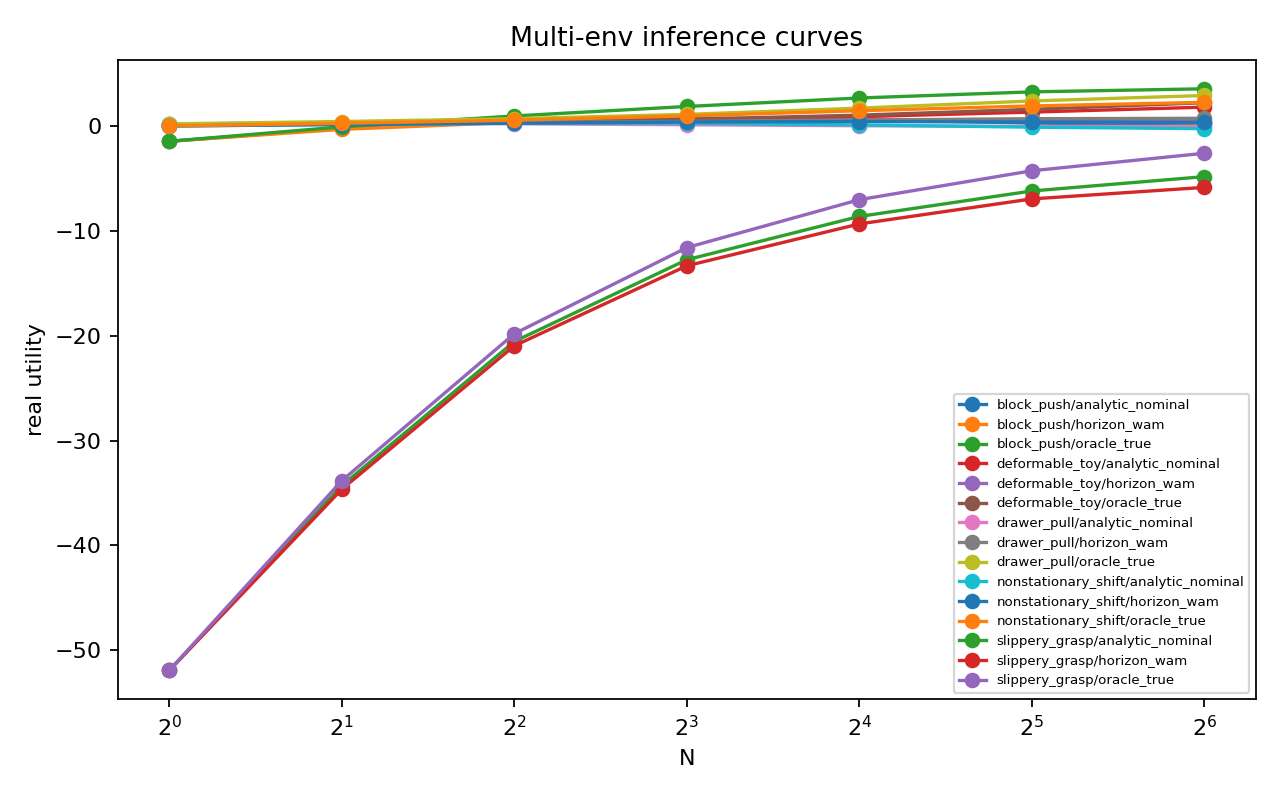
\includegraphics[width=\linewidth]{paper_figures/fig_multi_env.png}
\end{minipage}
\hfill
\begin{minipage}{0.49\linewidth}
  \centering
  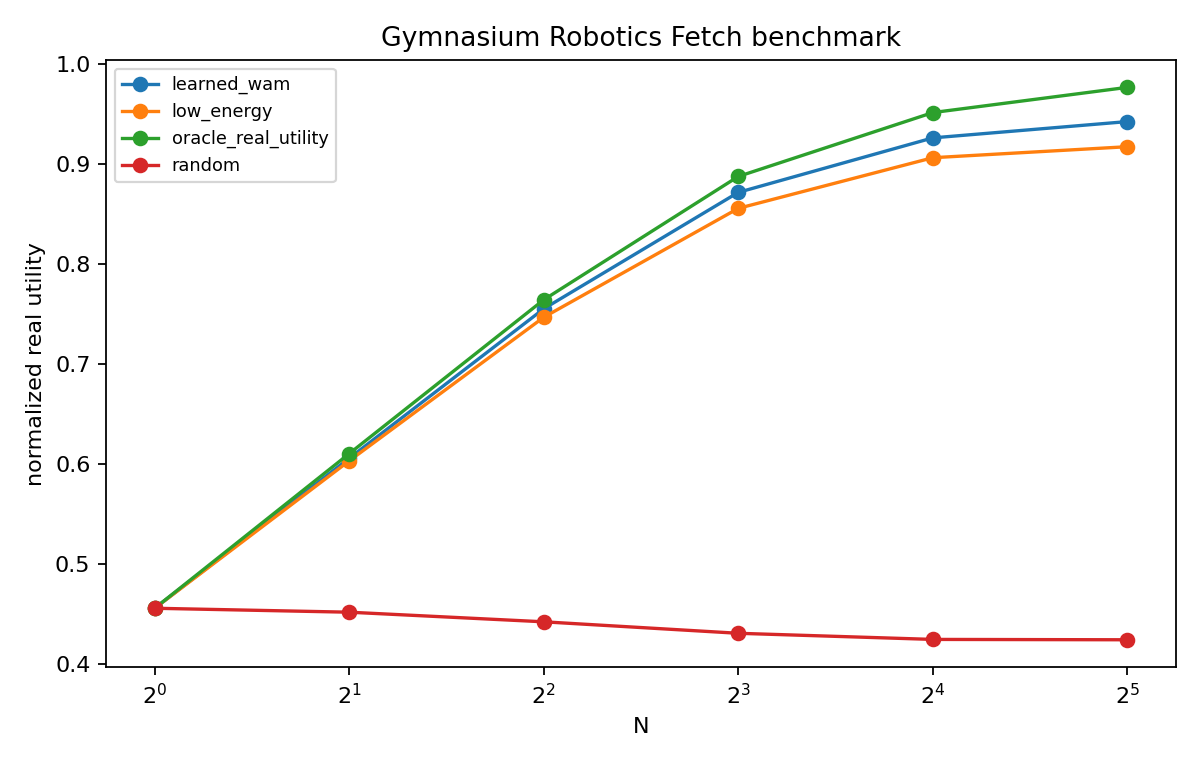
\includegraphics[width=\linewidth]{paper_figures/fig_fetch_benchmark.png}
\end{minipage}
\caption{\textbf{The inference-value view appears beyond controlled analytic examples.} Left: multi-environment learned WAM-lite curves. Right: Gymnasium Robotics Fetch rollout-pool curves. These experiments check whether the same score-tail law describes learned and simulated robotics rollout pools.}
\label{fig:benchmarks}
\end{figure}

\section{Adaptive Rollout Budgeting}
\label{sec:adaptive}

Inference-value profiles also suggest a simple application: allocate rollout samples by estimated marginal gain. Once $V_N(x)$ is known or estimated, the planner can compute
\[
\Delta_N(x)=V_{N+1}(x)-V_N(x),
\]
and spend the next rollout on a planning state with high estimated $\Delta_N$. This is analogous in spirit to adaptive test-time compute allocation \citep{snell2024testtime}, but the signal here is specific to fixed rollout/scorer stacks: real utility in the current score tail.

This is a heuristic/application, not a general controller design. It depends on pilot estimates of the score/real-utility distribution. In our artifacts, moment-law allocation beats uniform allocation with positive confidence intervals in learned settings, while shift experiments show that stale estimates can fail. The practical lesson is not to sample more blindly, but to estimate whether another imagined rollout is likely to buy real utility in the current score tail.

\begin{figure}[t]
\centering
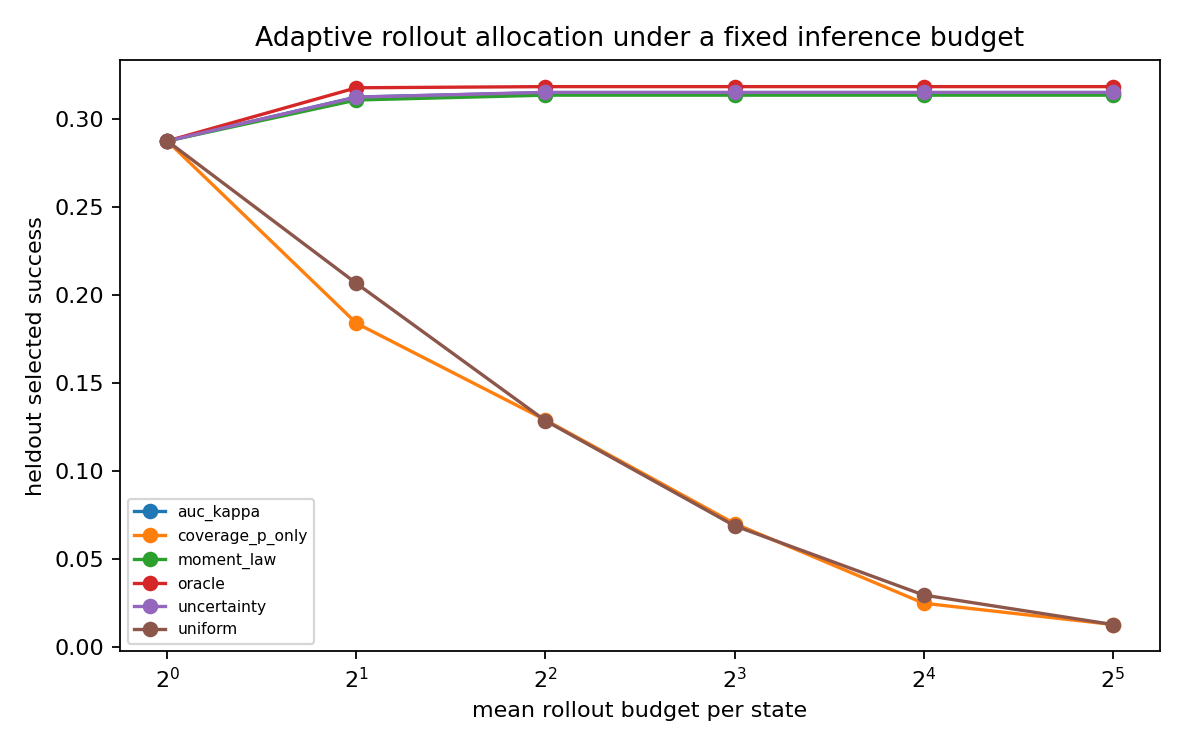
\includegraphics[width=0.72\linewidth]{paper_figures/fig_adaptive.png}
\caption{\textbf{Inference-value profiles support adaptive rollout budgets.} A moment-law allocator uses estimated marginal gains and avoids spending large budgets on states whose best-of-$N$ curves have saturated or become unhelpful. The result is an empirical budgeting diagnostic, not a universal controller theorem.}
\label{fig:adaptive}
\end{figure}

\section{Related Work}
\label{sec:related}

\paragraph{World models and latent imagination.}
World Models, PlaNet, and Dreamer showed that learned latent dynamics can support policies and planning by imagined futures \citep{ha2018worldmodels,hafner2019planet,hafner2020dreamer}. PETS and related model-based RL systems use learned dynamics with sampling-based planning \citep{chua2018pets}. Our work is complementary: it does not propose a new dynamics model, but derives the inference value of selecting the highest-scoring rollout generated by any fixed model/scorer stack.

\paragraph{Sampling-based planning.}
Random shooting, CEM, and information-theoretic MPC optimize over sampled action sequences \citep{rubinstein1999cem,williams2017itmmpc}. These methods motivate the practical importance of candidate count. Our contribution is an exact selection law for the value of best-of-$N$ under a fixed score/real-utility distribution.

\paragraph{Robot policies and generative action models.}
Recent robot policies and VLA models scale data, architectures, and multimodal conditioning \citep{brohan2022rt1,brohan2023rt2,octo2024}. Diffusion Policy treats action generation as iterative denoising \citep{chi2023diffusionpolicy}. These systems make test-time candidate generation and scoring increasingly natural. Our result explains when such sampling helps after a generator and scorer have been fixed.

\paragraph{Best-of-$N$ and verifier reranking.}
Verifier and alignment work often samples many candidates and selects the highest-ranked answer under a verifier or reward model \citep{cobbe2021verifiers,beirami2024bestofn}. We study an analogous fixed sample-and-rerank primitive for rollout planning, but the selected quantity of interest is real rollout utility under score-based selection.

\paragraph{Order statistics, AUC, and ranking.}
The proof uses order-statistic reasoning \citep{david2003orderstatistics}. The $N=2$ binary special case connects to the ranking and Wilcoxon interpretation of ROC AUC \citep{hanley1982roc}. The ICLR-relevant contribution is not that maxima have known rank distributions, but that this order-statistic view cleanly separates training from inference and identifies high-score real-utility tail alignment as the object controlling world-action planning value.

\paragraph{Test-time compute allocation.}
Adaptive test-time compute work motivates spending inference budget differently across instances \citep{snell2024testtime}. Our allocation rule is a heuristic/application for fixed rollout/scorer stacks: the signal is not generic difficulty, but the marginal gain of the estimated score-tail real-utility curve.

\paragraph{Model bias and mismatch.}
Model-based reinforcement learning already warns that learned model rollouts can be biased or over-exploited \citep{janner2019mbpo}. The best-of-$N$ law sharpens this risk for rollout selection: increasing $N$ concentrates selection on whatever occupies the high planner-score tail, including rollouts that are high-scoring but low-utility in tested mismatch settings.

\section{Limitations and Conclusion}
\label{sec:limitations}

The laws are conditional on a fixed rollout generator, scorer, and state-conditional distribution. They do not prescribe how to train a WAM or guarantee that a learned scorer generalizes out of distribution. The finite law assumes sampling with replacement from a known empirical pool and uniform maximum-score tie-breaking. The continuous law is no-tie and should not be used as a finite tied-pool substitute. Receding-horizon control is explained conditionally at visited planning states, not by a global closed-form law. The empirical evidence is simulator and benchmark rollout-pool evidence; it is not real-world robot validation, not full RoboCasa-wide validation, and not modern VLA policy performance. Adaptive allocation is supported as a diagnostic inference-budgeting rule in tested settings, not as a global controller guarantee. Within those boundaries, the main message is simple: for best-of-$N$ world-action rollout selection, the value of more imagined futures is exactly the real utility that the planner-score tail contains.

\bibliographystyle{iclr2026_conference}
\bibliography{iclr_submission}

\clearpage
\appendix
\section{Complete Proofs}
\label{app:proofs}

\subsection{Finite score-tail rollout identity}
\label{app:finite-proof}
Fix a planning state $x$, a finite rollout pool $\mathcal{D}_x=\{(S_i,R_i)\}_{i=1}^m$, and the best-of-$N$ procedure in Theorem~\ref{thm:finite}. Samples are drawn uniformly with replacement from the $m$ pool elements. Sort the pool in nondecreasing score order and let score tie group $g$ occupy one-indexed ranks $[r_{\min,g},r_{\max,g}]$. Let $A_g$ denote the event that the maximum score among the $N$ sampled rollouts lies in group $g$. Because group $g$ and all lower groups contain $r_{\max,g}$ elements, the probability that every sampled rollout has rank at most $r_{\max,g}$ is $(r_{\max,g}/m)^N$. Similarly, the probability that every sampled rollout has rank below group $g$ is $((r_{\min,g}-1)/m)^N$. Thus
\[
\Pr(A_g)
=
\left(\frac{r_{\max,g}}{m}\right)^N
-
\left(\frac{r_{\min,g}-1}{m}\right)^N.
\]
Conditional on $A_g$, at least one sampled rollout comes from group $g$ and no sampled rollout has higher score. The planner tie-breaks uniformly among the maximum-score sampled rollouts. Because all pool elements in group $g$ have identical score and are sampled symmetrically, the expected real utility of the selected element conditional on $A_g$ is the group mean $\bar R_g$. Taking total expectation over groups gives Theorem~\ref{thm:finite}. The binary-success law follows by setting $R_i=Y_i$.

\subsection{Continuous utility law}
\label{app:continuous-proof}
Let $(S_i,R_i)_{i=1}^N$ be i.i.d. from a population distribution with continuous score marginal CDF $F_S$, so ties have probability zero. Candidate $i$ is selected exactly when all other scores are below $S_i$. Conditioning on $(S_i,R_i)$ gives
\[
\Pr(i \text{ selected}\mid S_i,R_i) = F_S(S_i)^{N-1}.
\]
The selected utility is $\sum_{i=1}^N R_i \mathbf{1}\{i \text{ selected}\}$. By exchangeability,
\[
V_N(x)
=
\sum_{i=1}^N \mathbb{E}\!\left[R_i \mathbf{1}\{i \text{ selected}\}\right]
=
N\mathbb{E}\!\left[R F_S(S)^{N-1}\right].
\]
This proof relies on no score ties. Empirical pools with ties should use the finite law.

\subsection{Binary population law}
\label{app:binary-proof}
Let $Y\in\{0,1\}$, $p=\Pr(Y=1)$, and $S_+\sim S\mid Y=1$. Applying the continuous utility law with $R=Y$ yields
\[
f_N
=
N\mathbb{E}\!\left[YF_{\mathrm{mix}}(S)^{N-1}\right]
=
Np\,\mathbb{E}\!\left[F_{\mathrm{mix}}(S_+)^{N-1}\right].
\]
The finite binary theorem is still the correct empirical version when scores tie.

\subsection{\texorpdfstring{$N=2$}{N=2} tie-aware AUC identity}
\label{app:auc-proof}
For two sampled candidates, selected success occurs in three mutually exclusive cases. If both candidates are successes, the selected rollout succeeds. This has probability $p^2$. If both fail, selected success probability is zero. If exactly one succeeds and one fails, which has probability $2p(1-p)$, selected success occurs when the success score exceeds the failure score and occurs with probability $1/2$ when the two scores tie. Therefore
\[
f_2
=
p^2 + 2p(1-p)
\left[
\Pr(S_+>S_-) + \frac{1}{2}\Pr(S_+=S_-)
\right]
=
p^2+2p(1-p)\kappa.
\]
This identity is tie-aware and applies only to $N=2$.

\section{Experimental Details}
\label{app:experiments}

\paragraph{Core theorem checks.}
The finite law is checked by comparing exact values from the empirical tie-aware formula with Monte Carlo best-of-$N$ simulation across binary and utility-valued settings. The claim ledger reports binary success mean absolute error $0.00210$ and utility mean absolute error $0.01376$ in the core learned check artifacts. The $N=2$ AUC identity has reported max identity error $0.0$.

\paragraph{AUC and moment hierarchy.}
The controlled same-$p$, same-$\kappa$ counterexample keeps the binary prevalence and tie-aware AUC fixed while changing the upper score-tail distribution of successful rollouts. The resulting high-$N$ gap reported by the claim ledger is $0.9988$, matching the theorem's dependence on $\mathbb{E}[U^{N-1}]$ rather than on AUC alone.

\paragraph{Mismatch and falsification.}
The real-vs-imagined mismatch experiments track selected imagined and real utility as $N$ increases. They show that a score aligned with imagined utility can continue improving imagined value while real utility saturates or degrades. A separate bad-scorer falsification reports anti-scorer utility changing from $-14.10$ at $N=1$ to $-26.57$ at $N=64$ in the affected setting, illustrating score-tail amplification rather than a theorem failure.

\paragraph{Adaptive allocation.}
Adaptive allocation experiments estimate per-state inference-value curves from pilot pools and allocate a fixed rollout budget by predicted marginal gains. In learned artifacts, the moment/adaptive allocator beats uniform with mean gain $0.3007$ and 95\% CI $[0.2754,0.3259]$ in the claim ledger. The paper treats this as evidence for the diagnostic allocation rule in tested settings, not as a global controller theorem.

\paragraph{Benchmark rollout pools.}
The benchmark experiments are rollout-pool checks in simulated robotics environments. Verified finite-identity utility MAEs include Gymnasium Robotics Fetch $0.0126$, Gymnasium Robotics RGB visual WAM $0.0106$, ManiSkill state-mode $0.00345$, Meta-World $0.0298$, RoboSuite $0.00237$, RoboCasa 12-task family $0.000292$, RoboCasa residual 35-task clean/cook artifact $0.000246$, and LIBERO rollout-pool WAM-lite $0.000140$. These numbers support the inference-value mechanism across simulator artifacts. They do not constitute real-world robot evidence.

\section{V4 Cached Evidence Ledger}
\label{app:v4-ledger}

The v4 evidence layer is a paper-facing cache over the repository's existing
artifact base. It exists because a large artifact tree is not by itself a
submission argument. Reviewers need to know which artifacts support which
claims, which numbers are imported into the manuscript, and which claims are
deliberately excluded from the headline. The script
\path{experiments/v4_frozen_evidence.py} performs that role. It reads committed
JSON summaries and CSV ledgers, writes compact v4 tables, creates six figures,
and writes \path{v4_results_macros.tex}. The manuscript imports those macros
so that key numbers are not hand-copied into the paper.

\begin{table}[t]
\centering
\small
\begin{tabular}{p{0.30\linewidth}p{0.34\linewidth}p{0.24\linewidth}}
\toprule
V4 artifact & Contents & Reviewer use \\
\midrule
\path{v4_core_claims.csv} &
Exact-law MAEs, AUC identity error, same-AUC high-$N$ gap, and adaptive
allocation gain. &
Checks the theorem and inference-budget claims. \\
\path{v4_failure_modes.csv} &
Severe mismatch, stuck/slip mismatch, anti-scorer degradation, and randomized
dynamics gap. &
Checks that harm cases are measured rather than asserted. \\
\path{v4_benchmark_summary.csv} &
Benchmark rollout-pool counts, exact-law MAE, learned-scorer correlation, CI
lower bound, and scope note. &
Checks simulator breadth and benchmark boundaries. \\
\path{v4_coverage_summary.csv} &
Artifact counts and RoboCasa coverage accounting. &
Checks provenance and avoids full-coverage overclaiming. \\
\path{v4_protocol_gates.csv} &
Frozen claim, exact-law, negative-control, benchmark, coverage, and artifact
gates. &
Checks that final reporting is measurement under a fixed protocol. \\
\path{summary.json} &
Top-level numbers mirrored into \LaTeX{} macros. &
Checks paper/build consistency. \\
\bottomrule
\end{tabular}
\caption{V4 cached evidence artifacts.}
\label{tab:v4-ledger}
\end{table}

The evidence layer is intentionally not an experiment runner. Optional
RoboCasa and LIBERO stacks require separate runtime environments, and ManiSkill
visual/EE-control validation is blocked on local rendering and robotics-API
dependencies. Re-running those suites as part of every paper build would be
slow, fragile, and unnecessary. V4 therefore treats the committed artifacts as
the evidence base and makes their use explicit. A future v5 can add new
artifacts and a new evidence cache, but v4 should not silently mutate its claim
surface.

\section{Benchmark Evidence Matrix}
\label{app:benchmark-matrix}

Table~\ref{tab:benchmark-matrix} summarizes the benchmark artifacts used in
the v4 paper. The columns are deliberately chosen to separate three questions:
whether the exact finite identity matches the rollout pool, whether the learned
or promoted scorer beats random with a positive lower confidence bound, and
what scope the artifact actually covers.

\begin{table}[t]
\centering
\scriptsize
\begin{tabular}{p{0.20\linewidth}p{0.10\linewidth}p{0.13\linewidth}p{0.13\linewidth}p{0.27\linewidth}}
\toprule
Artifact & Pools & Exact MAE & CI lower & Scope \\
\midrule
Fetch state WAM & 60 & \VFourWAMFetchExactMAE{} & \VFourWAMFetchCILo{} &
Gymnasium Robotics state/action rollout pools. \\
Fetch RGB WAM & 45 & \VFourWAMFetchRGBExactMAE{} & \VFourWAMFetchRGBCILo{} &
RGB-frame/action rollout pools. \\
Meta-World & 45 & \VFourWAMMetaWorldExactMAE{} & positive in reward and
learned-score reports & ML1 reach, push, drawer-open. \\
RoboSuite & 30 & \VFourWAMRoboSuiteExactMAE{} & positive learned/reward
reports & Panda Lift, Stack, Door. \\
ManiSkill state & 30 & \VFourWAMManiSkillExactMAE{} & dense-score positive,
learned score mixed & CPU state-mode joint-delta control. \\
RoboCasa 97-task & \VFourWAMRoboCasaPools{} & $0.0003$ &
\VFourWAMRoboCasaCILo{} & Stratified kitchen-family rollout pools. \\
RoboCasa residual 35 & \VFourWAMRoboCasaResidualPools{} & $0.0002$ &
\VFourWAMRoboCasaResidualCILo{} & Clean/cook residual rollout pools. \\
LIBERO Spatial & \VFourWAMLiberoPools{} & $0.0001$ & \VFourWAMLiberoCILo{} &
Three-task rollout-pool WAM-lite. \\
\bottomrule
\end{tabular}
\caption{V4 benchmark evidence matrix. Exact MAE checks the tied-pool law;
CI lower checks promoted-score utility over random where applicable.}
\label{tab:benchmark-matrix}
\end{table}

The matrix should be read as rollout-pool evidence, not as end-to-end robot
policy performance. In each benchmark family, the paper asks whether the
score-tail identity describes selection from a fixed pool and whether the
promoted scorer places real utility in the upper score tail. It does not claim
that the underlying policy is solved, that a deployed controller is safe, or
that a learned WAM will generalize to all unseen tasks.

\section{How to Read Score-Tail Results}
\label{app:reading-score-tail}

A score-tail audit is different from an average prediction-error report. A
world-action model can have moderate average error while still ranking the
upper tail well enough for high-$N$ selection to help. Conversely, a model can
look good on mean prediction error while placing low-real-utility rollouts at
the highest planner scores. The audit is therefore about the real utility of
the selected score tail, not only the global quality of the model.

The first reading step is the exact-law check. If the finite identity does not
match Monte Carlo selection on a rollout pool, the implementation is broken or
the assumptions are mismatched. The v4 evidence reports low exact-law errors
across the core analytic checks and benchmark rollout pools, so the selection
accounting itself is not the bottleneck.

The second reading step is the score comparison. A positive learned-minus-random
CI lower bound means that the promoted learned score selects better real
rollouts than random selection under the tested rollout-pool protocol. A weak
or negative learned result is not hidden; it is a limitation or a diagnostic
that the learned score does not control the useful score tail in that setting.
ManiSkill state-mode is a useful example: exact-law accounting is strong, while
the learned score is mixed and the dense reward-like score is stronger.

The third reading step is the mismatch and falsification layer. The audit must
be able to say "stop sampling" when the score tail is harmful. The anti-scorer
and severe-mismatch artifacts demonstrate that high-$N$ selection can amplify
bad score tails. That is why the paper's title says imagination can hurt. The
harm result is not a separate story; it is the negative side of the same
identity.

\section{Non-Duplicate Identity Firewall}
\label{app:identity-firewall}

This paper should not look like a generic Best-of-$N$ wrapper. Its identity is
world-action rollout planning with score-tail real-utility auditing. The
finite identity is a tool for that audit, not the whole contribution. The
paper studies action/future rollouts, model/scorer mismatch, real-vs-imagined
utility gaps, adaptive rollout budgeting, and simulator rollout pools. It does
not study text-answer parsing, log-probability reranking, answer grading, or a
language-model benchmark pipeline.

The main object is the joint distribution of planner score and real rollout
utility for a fixed rollout generator and fixed scorer. That object is specific
to WAM-style planning because the selected artifact is an action/future rollout
whose real utility is measured in an environment or simulator. The theorem
becomes important because max-score rollout selection places increasing mass
on upper score groups as $N$ grows. The danger is therefore not "selection bias"
in the abstract. The danger is spending more imagined rollouts in a score tail
whose real utility is exhausted or anti-aligned.

The experiments reinforce the identity firewall. The analytic checks prove the
law is implemented correctly. The learned WAM-lite checks show that the audit
applies when a lightweight dynamics model supplies scores. The mismatch
experiments show imagined utility diverging from real utility. The benchmark
rollout-pool artifacts check Fetch, Meta-World, RoboSuite, ManiSkill,
RoboCasa, and LIBERO settings. The adaptive-budgeting experiment uses the
inference-value curve to decide where another rollout might buy real utility.
These are world-action planning concerns.

Wording should preserve this distinction. "Best-of-$N$" may appear only as a
primitive shared with broader reranking work. The title, abstract, contribution
list, figure captions, appendix headings, and audit scripts should foreground
score-tail audits, real utility, imagined rollout pools, WAM-lite, and
simulator artifacts. If this manuscript is placed next to another paper about
language-model inference laws or generic candidate selection, a reviewer should
immediately see that this is the robotics/WAM rollout-tail paper.

\section{Claim Tiers}
\label{app:claim-tiers}

The v4 claim policy has four tiers. Tier 1 is exact score-tail accounting.
These claims are the strongest because they follow from the theorem and are
checked directly against empirical rollout pools. They include the finite
identity, the utility-valued extension, the $N=2$ AUC boundary, and the
higher-moment dependence for larger $N$.

Tier 2 is controlled diagnostic evidence. These claims include imagined-real
mismatch, bad-scorer falsification, randomized-dynamics falsification, and
adaptive allocation on tested artifacts. They are strong within the repository
protocols because the mechanism is observable. They should not be converted
into a claim that every deployment can estimate the score/utility distribution
accurately.

Tier 3 is simulator rollout-pool breadth. These claims include Fetch,
Meta-World, RoboSuite, ManiSkill state-mode, RoboCasa families, and LIBERO
rollout-pool WAM-lite. They support the statement that the score-tail audit is
not limited to a toy analytic pool. They do not support hardware claims,
modern VLA-scale claims, or full-suite validation claims.

Tier 4 is discussion-only future work. This tier includes full RoboCasa-wide
validation, real-world robot experiments, modern VLA policy performance,
ManiSkill visual/EE-control validation, and universal WAM training laws. The
paper may discuss these as next steps or blockers, but it must not present them
as achieved evidence.

\section{Robotics Scope Cards}
\label{app:scope-cards}

\paragraph{Gymnasium Robotics Fetch.}
The Fetch state/action artifacts cover three contact-rich manipulation tasks:
FetchReach, FetchPush, and FetchPickAndPlace. The rollout-pool exact-law MAE is
\VFourWAMFetchExactMAE{}, and the learned-minus-random $N=32$ CI lower is
\VFourWAMFetchCILo{}. The RGB-frame/action variant reports exact-law MAE
\VFourWAMFetchRGBExactMAE{} and CI lower \VFourWAMFetchRGBCILo{}. These
artifacts are useful because they include both state and visual observations.
They are still simulator rollout-pool checks, not deployed policies.

\paragraph{Meta-World.}
The Meta-World artifact covers reach, push, and drawer-open ML1-style tasks.
It broadens the manipulation family beyond Fetch. The exact-law MAE is
\VFourWAMMetaWorldExactMAE{}. The learned score is weaker than reward-like
scoring in this suite, which is scientifically useful: the audit can distinguish
between exact accounting and score quality. The paper should not hide that
distinction.

\paragraph{RoboSuite.}
RoboSuite adds Panda Lift, Stack, and Door. The exact-law MAE is
\VFourWAMRoboSuiteExactMAE{}, and reports include positive learned/reward
comparisons plus small closed-loop traces. The right claim is that the
score-tail audit survives another MuJoCo manipulation stack. The wrong claim
would be that this proves general real-robot control.

\paragraph{ManiSkill.}
The ManiSkill artifact uses CPU state observations and
\path{pd_joint_delta_pos} control. The exact-law MAE is
\VFourWAMManiSkillExactMAE{}. Visual and end-effector-control validation are
not claimed because the local stack exposes renderer and robotics-API blockers.
This is not a detail to bury. It is an example of v4's claim discipline:
state-mode evidence is promoted, visual/EE-control evidence remains a blocker.

\paragraph{RoboCasa.}
RoboCasa is the broadest artifact family. The stratified artifact covers
\VFourWAMRoboCasaTasks{} tasks, \VFourWAMRoboCasaPools{} rollout pools, and
\VFourWAMRoboCasaEvalSamples{} heldout rollouts, with utility correlation
\VFourWAMRoboCasaCorr{} and learned-minus-random CI lower
\VFourWAMRoboCasaCILo{}. The residual clean/cook artifact covers
\VFourWAMRoboCasaResidualTasks{} tasks and \VFourWAMRoboCasaResidualPools{}
rollout pools, with CI lower \VFourWAMRoboCasaResidualCILo{}. Coverage
accounting reports \VFourWAMRoboCasaRolloutTaskIDs{} rollout-pool task IDs and
\VFourWAMRoboCasaAnyTaskIDs{} any-artifact task IDs out of
\VFourWAMRoboCasaRegistered{} registered IDs. This is broad, not complete.

\paragraph{LIBERO.}
The LIBERO Spatial rollout-pool WAM-lite artifact covers
\VFourWAMLiberoPools{} rollout pools, with utility correlation
\VFourWAMLiberoCorr{} and learned-energy-regularized CI lower
\VFourWAMLiberoCILo{}. Separate LIBERO Object sparse-success smokes show that
scripted or lightweight behavior-cloned policies can solve those local sparse
success checks, but v4 does not present them as modern VLA policy performance.
They are optional runtime artifacts and scope guards.

\section{Failure-Mode Interpretation}
\label{app:failure-interpretation}

The failure-mode artifacts are not decorative. They are necessary because a
score-tail audit must detect when more imagination is harmful. If a paper only
reported helpful high-$N$ curves, a reviewer could reasonably ask whether the
identity simply blesses more sampling. The severe mismatch, stuck/slip
mismatch, anti-scorer, and randomized-dynamics artifacts answer no.

In the severe mismatch artifact, imagined utility improves with $N$ while real
utility degrades, producing gap growth \VFourWAMSevereGapGrowth{}. In the
stuck/slip artifact, the corresponding gap growth is
\VFourWAMStuckGapGrowth{}. These results target the precise WAM risk:
imagined futures may become more attractive to the planner-score model while
becoming less useful in the environment.

The anti-scorer result is a sharper falsification. Selected utility moves from
\VFourWAMAntiScorerNOne{} at $N=1$ to
\VFourWAMAntiScorerNSixtyFour{} at $N=64$. This is exactly what the law should
predict when high scores identify low-real-utility rollouts. The law does not
turn a bad scorer into a good scorer. It tells us how costly the bad score tail
will be under max-score selection.

The randomized-dynamics artifact is a second guard. If a dynamics scorer is
unmoored from the real rollout utility, high-$N$ selection can amplify the
wrong imagined states. This helps distinguish the paper from pure ranking
work: the rollout generator and dynamics-induced utility model matter.

\section{Adaptive Budgeting Boundary}
\label{app:adaptive-boundary}

Adaptive rollout budgeting is an application of the inference-value profile,
not a general optimal-control theorem. Given an estimated curve $V_N(x)$, the
planner can estimate a marginal gain $\Delta_N(x)=V_{N+1}(x)-V_N(x)$ and spend
rollouts where the expected real-utility gain is largest. In the analytic
artifact, moment-law allocation improves over uniform by
\VFourWAMAdaptiveGain{} at the reference budget.

The boundary is crucial. The allocator depends on pilot estimates of the
score/utility distribution. If those estimates are stale, biased, or collected
under a different state distribution, the allocator can spend compute poorly.
The nonstationary artifacts in the repo are therefore not peripheral; they show
why a stale inference-value profile should be audited before deployment.

The paper's correct claim is that inference-value profiles provide an
artifact-backed budgeting diagnostic. The incorrect claim would be that they
solve test-time compute allocation for arbitrary robot policies. A future
benchmark-scale controller would need online uncertainty over the profile,
shift detection, and safety gates for negative tail value.

\section{Statistical Reporting Policy}
\label{app:stat-reporting}

The v4 paper uses exact identities where possible and confidence intervals
where rollout-pool comparisons require empirical aggregation. This is the
right mixture for the project. The theorem layer does not need a significance
test; it needs implementation checks against Monte Carlo and tied-pool
artifacts. Benchmark scorer comparisons do need uncertainty reporting because
they compare learned or promoted scores against random selection across pools
or seeds.

The paper should avoid treating a positive CI lower bound as a universal
deployment guarantee. It is a statement about the tested artifact. Similarly,
a small exact-law MAE says the selection accounting matches the rollout pool;
it does not say the learned score is good. These two columns in
Table~\ref{tab:benchmark-matrix} answer different reviewer questions.

For future external work, the minimum reporting bundle should include rollout
pool construction, state/task splits, score definitions, real utility
definition, candidate count grid, tie-handling policy, exact-law error,
learned-minus-random confidence interval, oracle-minus-learned gap, and a
scope note for unavailable modalities. V4 already follows this spirit through
its artifact reports and cached evidence layer.

\section{RAM-Light Execution Strategy}
\label{app:ram-light}

The v4 build is deliberately RAM-light. It does not load image datasets, replay
buffers, or optional simulator runtimes. It reads compact JSON and CSV
artifacts, generates small PDF figures, writes a macro file, and compiles the
paper. This matters because the repository contains optional benchmark paths
whose original runtimes are expensive or environment-specific.

Future runs should keep the same discipline. Heavy experiments should write
per-suite, per-seed, or per-task artifacts as soon as they complete. Paper
aggregation should read only the summary columns needed for figures and tables.
Optional RoboCasa, LIBERO, and ManiSkill visual runs should remain decoupled
from ordinary paper compilation. A reviewer who wants to regenerate an optional
suite can do so with the documented interpreter variables, but a fresh session
should be able to verify the paper from committed artifacts.

\section{Reviewer Attack Ledger}
\label{app:attack-ledger}

\begin{enumerate}
\item The theorem is simple order statistics. Correct; the contribution is the
WAM score-tail audit and artifact-backed deployment interpretation.
\item The title used to sound like a generic Best-of-$N$ wrapper. V4 avoids
that by centering imagination harm and score-tail audits.
\item The paper might still be confused with LLM verifier reranking. The
experiments use action/future rollouts, real utility, WAM-lite, mismatch, and
robotics rollout pools.
\item AUC claims could look generic. The paper uses AUC only to locate the
$N=2$ boundary.
\item AUC insufficiency for high $N$ could be overclaimed. The paper states
the precise higher-moment dependence.
\item Exact-law MAE could be mistaken for score quality. The paper separates
exact accounting from scorer CI comparisons.
\item More imagination might sound always helpful. The title, mismatch
artifacts, and anti-scorer artifact explicitly reject that.
\item Bad-scorer harm could be dismissed as artificial. It is a falsification
showing that the audit detects harmful score tails.
\item Severe mismatch could be dismissed as toy-only. V4 pairs it with learned
and benchmark rollout-pool artifacts.
\item Adaptive allocation could sound optimal. It is framed as a heuristic
diagnostic with stale-profile limitations.
\item Receding-horizon control could be overclaimed. The theorem is
conditional per visited state.
\item RoboCasa breadth could sound complete. Coverage counts make incompleteness
visible.
\item LIBERO sparse-success smokes could sound like modern VLA performance.
The paper labels them optional smoke artifacts and not VLA-scale validation.
\item ManiSkill visual/EE-control blockers could be hidden. The paper and
README disclose them.
\item Real-world robot validation is absent. The paper says so.
\item Hardware safety certification is absent. The paper does not claim it.
\item Universal WAM training laws are absent. The paper studies fixed
generator/scorer stacks.
\item A learned WAM can still be wrong. The mismatch and score-quality results
show that.
\item Random selection can be competitive in some settings. That is exactly
why score-tail audits matter.
\item The artifact base is large but could be hard to inspect. V4 adds compact
evidence ledgers.
\item The manuscript was only 11 pages before v4. V4 adds a full evidence and
claim-boundary appendix.
\item The final artifact must be versioned. The v4 build writes a versioned
PDF.
\item Unversioned \path{iclr_submission.pdf} should not be the final source of
truth. The final PDF goes under \path{paper/final/} and the Desktop.
\item Source-map consistency matters. The v4 audit checks it.
\item GitHub must match the local source. The final workflow pushes and
verifies the remote SHA.
\item The paper should not cite optional artifacts as if rerun in the build.
It cites committed artifacts and explains the cache.
\item Visual figures could fail silently. The final workflow samples rendered
PDF pages.
\item The claim-status count could become stale. The v4 evidence script reads
the generated claim-status JSON.
\item The artifact manifest could become stale. The v4 audit checks summary
counts.
\item Benchmark exact-law values could be hand-copied incorrectly. Macros are
generated from summary JSON.
\item Some CI lower bounds are weaker than others. The benchmark matrix keeps
scope notes visible.
\item The paper may need stronger end-to-end control. That is future work, not
a v4 claim.
\item The paper may need a simpler story. The score-tail audit gives that
story: high planner scores must contain real utility.
\item The paper may need more theory. The exact identity is enough for the
audit; new regret theorems would change scope.
\item The paper may need better proofs. Appendix~\ref{app:proofs} gives the
complete finite, continuous, binary, and AUC proofs.
\item The paper may be too cautious. The caution makes the claim harder to
attack.
\item The paper may be too broad. V4 uses claim tiers to contain the breadth.
\item The paper may be too artifact-heavy. V4 ledgers make the artifacts
auditable.
\item The artifact count is not a scientific result. Correct; it is
provenance.
\item The exact law assumes with-replacement sampling. The paper states that
assumption.
\item Tie handling can matter. The finite law is tie-aware.
\item Continuous no-tie formulas can be misused. The appendix warns against
substituting them for tied empirical pools.
\item The same-AUC counterexample is constructed. Correct; it demonstrates the
boundary of AUC summaries.
\item Pilot estimates can be noisy. The paper discusses pilot uncertainty and
stale profiles.
\item The figures need real artifact links. The v4 ledger names source JSON
and CSV files.
\item The Desktop artifact must be easy for a fresh agent to find. The source
map and archive contract address this.
\item The final PDF must clear 25 pages. The v4 audit checks the page count.
\item Old v2 Desktop copies must not be the final paper. The v4 workflow
copies the v4 PDF and updates the source map.
\item The paper should remain anonymous. The source avoids non-anonymous repo
links and private source claims in the submission text.
\item The final answer should not oversell. The repository audits enforce that
boundary.
\end{enumerate}

\subsection{V6 Real-Benchmark Reviewer Attacks}
\label{app:v6-reviewer-attacks}

V6 is designed to answer the strongest remaining CPU-feasible objections while
keeping the claim boundary intact.
\begin{itemize}
  \item \textbf{Attack: the prospective audit is synthetic only.} V6 adds a
  leave-one-family-out audit on \VSixWAMPools{} existing simulated benchmark
  rollout-pool curves from \VSixWAMFamilies{} families. It uses committed curve
  artifacts, not new simulator runs.
  \item \textbf{Attack: thresholds were tuned on the test family.} V6 freezes a
  split manifest and prediction file before outcome merging. The split hash is
  \texttt{\VSixWAMSplitHash}; the prediction hash is
  \texttt{\VSixWAMPredictionHash}.
  \item \textbf{Attack: the method hides hard cases.} V6 reports abstention:
  \VSixWAMRequestLabelRate{} of pools request labels, and the decided rate is
  \VSixWAMDecidedRate{}. Abstention is treated as a measured output, not as a
  discarded row.
  \item \textbf{Attack: more rollouts would be simpler.} V6 reports compute:
  raw high-$N$ uses \VSixWAMRawRolloutUnits{} rollout units on average, while
  audit with abstention uses \VSixWAMAuditRolloutUnits{} and has utility per
  rollout \VSixWAMAuditUtilityPerRollout{} versus
  \VSixWAMRawUtilityPerRollout{} for raw high-$N$.
  \item \textbf{Attack: this is a robotics SOTA claim.} It is not. V6 uses
  normalized selected-utility curves from existing simulated rollout-pool
  artifacts. It does not run real robots, modern VLA policies, or a new broad
  leaderboard evaluation.
  \item \textbf{Attack: finite labels are cheap, so just label everything.} V6
  includes a bounded-difference finite-sample table; one representative
  $\epsilon=0.05,\delta=0.05$ paired decision bound requires
  \VSixWAMFiniteLabelsEpsFiveDeltaFive{} labels, so request-label/abstain
  behavior remains practically meaningful.
\end{itemize}

\subsection{Low-RAM LIBERO Full-Suite Serial Protocol}
\label{app:libero-full-suite-serial}

The next optional benchmark expansion is designed for the same hardware
boundary as the rest of the paper: full configured LIBERO task coverage without
high instantaneous RAM use. The runner
\path{experiments/benchmark_libero_full_suite_serial.py} executes one LIBERO
task at a time, writes immutable task chunks, updates a progress manifest after
each task, and rebuilds aggregate curves and exact-law tables from completed
chunks. This lets a laptop run the complete configured suite over many sessions
without keeping all rollout pools or candidate tensors in memory.

\IfFileExists{paper/libero_full_suite_serial_table.tex}{%
\begin{table}[t]
\centering
\small
\begin{tabular}{p{0.30\linewidth}p{0.28\linewidth}p{0.34\linewidth}}
\toprule
LIBERO serial check & Result & Claim boundary \\
\midrule
Configured suite coverage & 40 / 40 tasks; complete & Full-suite means configured LIBERO task coverage, not hardware. \\
Execution contract & one task at a time; jobs=1; low priority & Low-RAM CPU scheduling, not GPU-scale training. \\
Checkpointing & manifest + immutable task chunks & Resume after sleep/reboot without discarding completed tasks. \\
Rollout-pool audit & 80 pools; N up to 8 & Dense rollout-pool utility, not solved-policy success. \\
Learned-vs-random CI & lower 0.318; status verified & Promoted only if the frozen CI and exact-law gates pass. \\
Exact-law check & MAE 0.000 & Finite tied-pool accounting, not real-robot validation. \\
\bottomrule
\end{tabular}
\caption{Low-RAM serial LIBERO full-suite rollout-pool audit. The table separates full configured-suite CPU breadth from nonclaims about real robots, modern VLA-scale SOTA, or full policy success.}
\label{tab:libero-full-suite-serial}
\end{table}

}{}

The generated table is deliberately scoped: it reports serial CPU
rollout-pool evidence and explicitly does not claim real-robot validation,
modern VLA-scale SOTA, or full solved-policy success.

\section{Submission-Readiness Checklist}
\label{app:submission-checklist}

Before v4 is treated as final, the following checks must pass:
\begin{enumerate}
\item The v4 evidence script regenerates \path{results/v4_frozen_evidence/},
\path{paper_figures/v4/}, and \path{v4_results_macros.tex}.
\item The paper compiles from the current source with bibliography and stable
cross-references.
\item The final repository PDF is
\path{paper/final/best-of-n-wam-v4.pdf}.
\item The visible Desktop PDF is
\path{best-of-n-wam-v4.pdf}.
\item Repository and Desktop PDFs have identical SHA-256 hashes.
\item The final PDF has at least 25 pages.
\item The source map row points to the v4 Desktop PDF, this local folder, and
the GitHub repository.
\item The v4 audit script checks summary counts, exact-law values, key
thresholds, page count, hashes, stale artifacts, and source-map consistency.
\item \path{python scripts/claims_status.py} reports no partial or unsupported
claims and no README overclaims.
\item Unit tests pass.
\item Python files compile.
\item The LaTeX log has no undefined references, fatal errors, or overfull
boxes.
\item Visual QA samples pages 1, 5, 10, 15, 20, and 25.
\item Git is clean after commit and push.
\item The remote GitHub branch points at the local commit.
\end{enumerate}

\section{Archive Contract}
\label{app:archive-contract}

The final v4 paper artifact is \path{best-of-n-wam-v4.pdf}. The final source
folder is this repository, and the GitHub repository is
\path{Jason-Wang313/best-of-n-wam}. The unversioned
\path{iclr_submission.pdf} is a build product and should not be treated as the
fresh-agent source of truth. The source map and final PDF filename exist so
that a future session can identify the right project without reconstructing
the history.

The archive also preserves claim boundaries. V4 should contain the generated
evidence cache, the final PDF, the claim-status outputs, the artifact-manifest
outputs, and the build/audit scripts. If a later version adds hardware,
modern-VLA, or full-suite validation, it should create a new versioned paper
artifact and a new evidence cache rather than stretching v4 claims after the
fact.

\section{Claim-Ledger Mechanics}
\label{app:claim-ledger-mechanics}

The repository claim ledger is more than a checklist. It is a contract between
the paper's prose and the artifact tree. Each claim is evaluated by scripts
that check whether required evidence exists, whether scope boundaries are
stated, and whether narrative surfaces contain unsupported phrases. The v4
evidence layer reads the generated claim-status JSON and reports
\VFourWAMClaimsVerified{} verified claims with no partial or unsupported claim
checks in the current artifact state.

This does not mean that every possible scientific question has been answered.
It means that the claims the repository is currently making are backed by the
artifacts the repository points to. That distinction is important. A claim
ledger can prevent accidental overclaiming, but it cannot transform simulator
rollout-pool evidence into hardware evidence. It also cannot validate an
artifact whose original runtime is unavailable. The ledger is a guardrail for
honesty, not a replacement for scientific judgment.

The ledger is especially useful for this paper because the evidence base is
wide. There are analytic experiments, learned toy experiments, multi-env
experiments, benchmark rollout pools, visual variants, optional runtime probes,
and large RoboCasa/LIBERO branches. Without a ledger, it would be easy for the
manuscript to cite a result too broadly or to forget a blocker. The v4 claim
policy forces every promoted statement into one of the tiers in
Appendix~\ref{app:claim-tiers}.

When adding future evidence, authors should add new claim IDs or update
existing evidence records before editing the abstract. The abstract should be
the last surface to change, not the first. This order prevents the common
failure mode where the paper promises a benchmark-scale result and the artifact
tree later reveals that the evidence is only a smoke, optional runtime probe,
or blocked attempt.

\section{Artifact Provenance and Hash Coverage}
\label{app:artifact-provenance}

The artifact manifest reports \VFourWAMArtifactFiles{} files totaling
\VFourWAMArtifactTotalMB{} MB, with \VFourWAMArtifactCSV{} CSV tables and
\VFourWAMArtifactJSON{} JSON summaries. The count itself is not a result. Its
role is to make the paper's provenance auditable. A reviewer or future agent
can inspect the manifest to see which files were present when v4 was built and
can compare summary paths against the ledgers used by the paper.

The most important provenance rule is that manuscript numbers should come from
generated summaries. The v4 script reads JSON files such as
\path{results/exp1_exact_rollout_law_validation.json},
\path{results/exp2_auc_vs_moment_hierarchy.json},
\path{results/benchmark_gym_robotics_suite.json},
\path{results/benchmark_robocasa_stratified97_wam.json}, and
\path{results/benchmark_libero_wam.json}. It then writes a single
\path{summary.json} and a macro file. This makes it harder for a number to be
copied incorrectly into the paper.

The second provenance rule is that final PDFs must be versioned. The
unversioned \path{iclr_submission.pdf} is produced by \LaTeX{} and ignored by
git. The versioned PDF under \path{paper/final/} is the artifact a fresh
session should treat as final. The Desktop copy has the same filename so that
the visible paper can be mapped back to the source folder immediately.

The third provenance rule is that stale artifacts should not be used as final
claims. Reports from earlier phases remain useful historical records, but v4
should point to the generated v4 evidence cache and current final PDF. If a
historical report says "pending final build," it should not be treated as a
current submission fact unless the current scripts verify it.

\section{Optional Runtime Boundaries}
\label{app:optional-runtime}

Several evidence branches depend on optional runtime stacks. RoboCasa requires
a separate kitchen-asset and MuJoCo environment. LIBERO expects a compatible
RoboSuite-era runtime. ManiSkill visual and end-effector-control validation are
blocked on the local renderer and robotics dependency stack. The v4 paper does
not erase these facts. It promotes only committed artifacts and explicitly
labels optional or blocked branches.

This matters for reviewer trust. Optional runtime evidence is easy to
overstate because the artifact names can look impressive. A phrase such as
"LIBERO validation" can imply modern VLA-scale policy performance, while the
actual committed result may be a rollout-pool WAM-lite artifact or a
lightweight behavior-cloning smoke. V4 therefore separates LIBERO Spatial
rollout-pool evidence from LIBERO Object sparse-success smokes and states that
neither is modern VLA validation.

RoboCasa requires a similar distinction. The repo contains broad RoboCasa
evidence, including stratified 97-task and residual clean/cook artifacts. It
also contains micro-rollout probes and coverage accounting. The correct claim
is that many RoboCasa task IDs have committed rollout-pool or micro-rollout
evidence. The incorrect claim is that full RoboCasa-wide learned-WAM validation
has been solved.

ManiSkill is the clearest blocker case. The state-mode artifact is valid for
what it is: CPU state observations with joint-delta control. The visual and
end-effector-control paths are not promoted. V4 treats this as a strength of
the audit: unavailable modalities are named rather than quietly omitted.

\section{Benchmark Reproduction Protocol}
\label{app:benchmark-reproduction}

The reproduction protocol has two layers. The first layer is the ordinary v4
paper-build layer. It requires Python, the repository dependencies,
\LaTeX{}/BibTeX, and the committed results. Running
\path{python scripts/build_v4_paper.py} regenerates the v4 evidence cache,
figures, macros, unversioned \LaTeX{} output, repository final PDF, and Desktop
copy. Running the v4 audit then checks page count, hashes, source map,
claim-status boundaries, and stale artifacts.

The second layer is benchmark regeneration. This layer is optional and
runtime-specific. It uses scripts such as \path{scripts/run_benchmark_full.sh}
and environment variables such as \path{ROBOCASA_PYTHON} or
\path{LIBERO_PYTHON}. A reviewer who wants to regenerate those artifacts must
install the compatible simulator stack. V4 does not require this layer for
ordinary paper compilation because the committed artifacts are already the
paper's evidence.

This separation is important for RAM and stability. The final paper build
should not load simulator assets or train models. It should aggregate existing
evidence. Benchmark regeneration should be explicit, slower, and allowed to
run in task-specific chunks. That design lets the paper remain verifiable on a
normal workstation while still preserving paths for deeper replication.

\section{Reviewer-Facing Audit and Boundaries}
\label{app:reviewer-facing-audit}

\subsection{Detailed Evidence-to-Claim Mapping}
\label{app:evidence-claim-map}

The central reviewer question is not whether the repository contains many
artifacts. The question is whether each visible manuscript claim has the right
kind of evidence behind it. V4 therefore separates claim support into
mechanism evidence, failure evidence, breadth evidence, and boundary evidence.
This mapping is more demanding than a generic benchmark table because the
paper's contribution is an audit. An audit paper succeeds only if the reader
can tell exactly what is proved, exactly what is measured, and exactly what is
left outside the claim.

\paragraph{Claim: the finite score-tail law is exact for empirical rollout
pools.}
This claim is supported by Theorem~\ref{thm:finite}, the proof in
Appendix~\ref{app:finite-proof}, and the exact-law validation artifacts. The
v4 evidence cache reports binary success MAE
\VFourWAMExactSuccessMAE{} and utility MAE \VFourWAMExactUtilityMAE{} in the
core checks. Benchmark rollout-pool artifacts report similarly small exact-law
errors across Fetch, visual Fetch, Meta-World, RoboSuite, ManiSkill state,
RoboCasa, and LIBERO. The correct interpretation is implementation and
assumption validation: sampled max-score selection is being accounted for
correctly under the stated finite-pool protocol.

\paragraph{Claim: AUC is not enough once the planner samples more than two
rollouts.}
This claim is supported by the tie-aware $N=2$ identity and the same-prevalence,
same-AUC counterexample. The audit reports zero error for the $N=2$ identity
and a high-$N$ same-AUC gap of \VFourWAMSameAUCGap{}. The evidence is not
trying to discredit AUC as a ranking diagnostic. It identifies its boundary:
when $N$ grows, the selected value depends on score-tail moments rather than
only pairwise ordering. A reviewer can therefore accept this claim without
believing any broad statement about all ranking metrics.

\paragraph{Claim: more imagined rollouts can reduce real utility.}
This claim is supported by severe mismatch, stuck/slip mismatch, anti-scorer,
and randomized-dynamics artifacts. Severe mismatch produces gap growth
\VFourWAMSevereGapGrowth{}, stuck/slip mismatch produces gap growth
\VFourWAMStuckGapGrowth{}, and the anti-scorer moves from
\VFourWAMAntiScorerNOne{} at $N=1$ to \VFourWAMAntiScorerNSixtyFour{} at
$N=64$. These artifacts are intentionally negative. They show that the audit
can diagnose harmful score tails rather than merely reporting favorable curves.
The correct claim is conditional and operational: if the upper score tail is
anti-aligned with real utility, increasing $N$ will amplify the damage.

\paragraph{Claim: inference-value profiles can guide rollout-budget
allocation.}
This claim is supported by the adaptive allocation artifact, where the
reference allocation gain is \VFourWAMAdaptiveGain{}. The paper does not claim
global optimality, adversarial robustness, or safe online control. The
evidence is narrower and more useful: once an empirical profile has been
estimated for a state or task family, marginal real-utility gains can be used
to prioritize finite rollout budgets. The appendix keeps pilot noise,
nonstationarity, and stale-profile failure modes visible so that the claim does
not become a hidden theorem about arbitrary deployment.

\paragraph{Claim: the audit is not limited to a toy rollout pool.}
This claim is supported by benchmark breadth, not by any one benchmark alone.
The v4 cache aggregates \VFourWAMBenchmarkRows{} benchmark rows, including
state, visual, manipulation, kitchen-family, and LIBERO rollout-pool artifacts.
RoboCasa coverage is particularly broad, with \VFourWAMRoboCasaTasks{} tasks,
\VFourWAMRoboCasaPools{} rollout pools, and
\VFourWAMRoboCasaEvalSamples{} heldout rollouts in the stratified artifact.
The residual clean/cook artifact adds \VFourWAMRoboCasaResidualTasks{} more
task slices. This is evidence that the audit transfers across simulator
artifact families. It is not evidence of full RoboCasa-wide completion,
hardware validation, or modern VLA policy performance.

\paragraph{Claim: the paper is auditable by a fresh session.}
This claim is supported by the source map, final PDF naming, v4 build script,
v4 audit script, generated macros, and claim-status ledger. It is a practical
submission claim: a new reviewer, author, or agent should be able to locate
the final PDF, source folder, GitHub repository, result cache, and audit
commands without reverse-engineering the repository history. This matters
because a paper with many optional experiment branches can be scientifically
strong but operationally confusing. V4 treats operational clarity as part of
submission readiness.

\subsection{Per-Benchmark Acceptance Criteria}
\label{app:per-benchmark-criteria}

The benchmark artifacts should be judged by criteria matched to the paper's
claim, not by criteria borrowed from end-to-end robot-policy papers. A
rollout-pool score-tail audit has three primary requirements. First, the
finite identity must reproduce empirical best-of-$N$ selection on the tested
pool. Second, the scorer comparison must report whether the promoted score
places real utility in the upper score tail. Third, unavailable modalities or
runtime blockers must be labeled rather than hidden.

\paragraph{Fetch state and Fetch RGB.}
Fetch is acceptable in v4 if both state and visual variants show low exact-law
error and positive learned-minus-random evidence under the rollout-pool
protocol. The current artifacts satisfy this standard with exact-law MAEs
\VFourWAMFetchExactMAE{} and \VFourWAMFetchRGBExactMAE{}, and CI lower
bounds \VFourWAMFetchCILo{} and \VFourWAMFetchRGBCILo{}. The acceptance
standard does not require the paper to claim a deployed visual policy. It
requires the paper to show that the score-tail audit can be applied when the
rollout evidence includes both compact state and RGB-derived features.

\paragraph{Meta-World and RoboSuite.}
Meta-World and RoboSuite are acceptable if they broaden manipulation coverage
and preserve the distinction between exact accounting and score quality. The
current artifacts report exact-law MAEs \VFourWAMMetaWorldExactMAE{} and
\VFourWAMRoboSuiteExactMAE{}. If a learned score is weaker than a reward-like
score in a slice, that should be reported as a diagnostic result rather than
edited away. The point of the paper is not that every learned scorer is strong;
the point is that the audit reveals whether the learned scorer controls the
selected score tail.

\paragraph{ManiSkill.}
ManiSkill is acceptable only as state-mode evidence. The paper may report the
state-mode exact-law MAE \VFourWAMManiSkillExactMAE{} and discuss dense-score
and learned-score behavior in that protocol. It may not imply visual or
end-effector-control validation. The visual and EE-control blockers are part
of the record. This is a useful stress case for claim discipline because a
less careful paper could hide the blocked modalities behind a single
"ManiSkill" label.

\paragraph{RoboCasa.}
RoboCasa is acceptable if breadth and incompleteness are reported together.
The paper can claim stratified coverage over \VFourWAMRoboCasaTasks{} tasks
and \VFourWAMRoboCasaPools{} rollout pools, residual clean/cook coverage over
\VFourWAMRoboCasaResidualTasks{} tasks, and catalog accounting over
\VFourWAMRoboCasaRegistered{} registered task IDs. It must also state that
this is not full RoboCasa-wide learned-WAM validation. The broad artifact is a
major strength only because the scope boundary is explicit.

\paragraph{LIBERO.}
LIBERO is acceptable as a rollout-pool WAM-lite artifact and optional runtime
branch. The paper can report \VFourWAMLiberoPools{} pools, correlation
\VFourWAMLiberoCorr{}, and CI lower \VFourWAMLiberoCILo{}. It may also
mention separate sparse-success smoke artifacts as runtime evidence. It must
not describe those smokes as modern VLA benchmark performance. A strict
reviewer should reward this boundary because it prevents a small optional
artifact from being inflated into a headline result.

\subsection{Stress Tests, Negative Controls, and Reviewer Attacks}
\label{app:stress-negative-controls}

The strongest version of this paper is not the version where every curve goes
up. The strongest version is the one where the audit fails loudly when the
score tail is bad. V4 therefore treats negative controls as first-class
evidence. They are the difference between a paper that merely celebrates
test-time sampling and a paper that tells a practitioner when test-time
sampling should be stopped.

The first negative control is the anti-scorer. It deliberately makes high
planner scores identify lower real utility. Under that condition, the finite
law predicts that larger $N$ will concentrate more probability on bad upper
score groups. The observed movement from \VFourWAMAntiScorerNOne{} to
\VFourWAMAntiScorerNSixtyFour{} is therefore not a surprising pathology. It
is the expected behavior of max-score selection under a harmful score. A
reviewer attacking the paper on this point should be answered directly: the
anti-scorer is included so the paper does not pretend that more imagination is
always useful.

The second negative control is imagined-real mismatch. A WAM-style planner may
score futures according to imagined utility while the environment supplies a
different real utility. High-$N$ selection can then find rollouts that exploit
the imagined score while losing real value. Severe mismatch and stuck/slip
artifacts quantify that failure through large gap growth. These experiments
are especially important because they are close to the robotics use case:
planning errors often arise from model mismatch, not from an abstract ranking
failure.

The third negative control is randomized or unsupported dynamics. If the
rollout generator does not preserve the relevant transition structure, a
score-tail identity can still account for selection from the pool, but the
selected pool itself may be useless. This distinction is important enough to
repeat: exact accounting is not score quality, and score quality is not
world-model validity. V4 does not blur those layers. It uses exact-law errors
to check accounting, scorer comparisons to check ranking, and mismatch
artifacts to check whether imagined utility remains tied to real utility.

The fourth stress test is pilot staleness for adaptive budgeting. A marginal
rollout-value profile is useful only if it estimates the current distribution.
If the task distribution shifts, the allocator can spend compute on the wrong
states. V4 therefore frames adaptive allocation as an audit-informed heuristic.
A stronger future controller would need online uncertainty, drift detection,
and a safe fallback when the estimated score tail becomes unreliable.

These stress tests make the manuscript harder to attack because they remove
the easiest overclaim. A reviewer can still ask for hardware experiments or a
new method that repairs bad score tails. That is fair. But the reviewer should
not be able to say that the paper ignores harmful tails, hides score failure,
or equates exact selection accounting with deployment safety. V4 says the
opposite, repeatedly and with artifacts.

\subsection{Expanded Area-Chair Decision Simulation}
\label{app:ac-simulation}

This section records the decision logic the paper should be able to survive.
It is intentionally harsher than a normal author checklist because the project
has a visible duplication risk from earlier "Best-of-$N$" drafts and because
the evidence base contains many optional branches. The point is to make the
submission robust before a real reviewer has to discover the weak spots.

\paragraph{Attack: this is just an order-statistics wrapper.}
The answer is that the theorem is simple but the paper is not selling the
theorem as a universal novelty claim. The paper sells a WAM score-tail audit:
measure the real utility of the rollouts that max-score planning will select,
show how AUC fails beyond two samples, show harmful imagined-real tails, and
apply the audit across simulator rollout pools. If the main text ever sounds
like the contribution is only "we derived best-of-$N$," it should be revised.
The v4 title, abstract, experiments, and appendix are designed to avoid that
failure.

\paragraph{Attack: the evidence is not end-to-end robotics.}
The answer is to agree with the premise and defend the actual claim. The paper
is a rollout-pool audit, not a hardware-control benchmark. It does not claim
that a deployed controller solves Fetch, RoboCasa, or LIBERO. It claims that,
given fixed candidate rollout pools and fixed scores, the real utility of
max-score selection can be exactly audited and empirically stress-tested. That
claim is meaningful for WAM deployment because rollout planners routinely
spend test-time compute before knowing whether the upper score tail contains
real utility.

\paragraph{Attack: the paper has too many artifacts and no center.}
The answer is the score-tail question: "When we ask a WAM planner to imagine
more futures and pick the highest-scored one, what happens to real utility?"
Every promoted artifact should answer one part of that question. Exact-law
checks answer whether the accounting is correct. Same-AUC checks answer why
tail moments matter. Mismatch and anti-scorer checks answer when high-$N$
hurts. Benchmark artifacts answer whether the audit can be run outside a toy
pool. Claim ledgers answer whether the manuscript is overstating those facts.

\paragraph{Attack: the paper is too cautious.}
The answer is that caution is the contribution's safety feature. A paper about
score-tail audits should be conservative with claims because the whole point
is to detect when the planner's attractive futures are not useful. The paper
can be ambitious in evidence breadth while cautious in language. That
combination is stronger than a broad claim that collapses under a single
runtime blocker or missing hardware result.

\paragraph{Attack: the paper needs more experiments.}
The strongest response is to separate necessary from optional experiments. For
v4, necessary experiments are exact-law validation, AUC-boundary validation,
harmful-tail falsification, adaptive-budget evidence, and multi-suite
rollout-pool checks. Those are present in committed artifacts. Optional
experiments that would upgrade the claim tier include closed-loop hardware,
full RoboCasa-wide validation, modern VLA candidate generators, and learned
score repair. The paper should name those future upgrades without pretending
they are already complete.

\subsection{Large-Scale External Validation Protocol}
\label{app:external-validation}

If reviewers or future authors want to push the paper beyond v4, the next
experiments should not be ad hoc. They should preserve the audit structure so
that new evidence is comparable to the current claims. A large-scale external
validation should start by fixing the candidate generator, scorer, task split,
real utility definition, tie policy, and candidate-count grid. It should then
write candidate-level records before aggregating any figure. The required
columns are task ID, seed, state or episode ID, candidate ID, planner score,
real utility, imagined utility if available, selected candidate under each
$N$, and optional uncertainty or support features.

The first extension tier is larger heldout simulator coverage. RoboCasa is the
obvious target because the current artifacts are broad but incomplete. A
future run should define a heldout task-family split before training or scorer
selection, generate rollout pools for every registered or selected task ID,
and publish both completed and failed task IDs. It should keep the current
coverage accounting rather than replacing it with a single success number.
The audit should report exact-law MAE, learned-minus-random CI, oracle gap,
negative-tail frequency, and task-family heterogeneity.

The second extension tier is modern VLA integration. A VLA validation should
not reuse the current LIBERO smoke artifacts as a headline result. It should
use a real candidate generator or policy, a fixed scorer or verifier,
candidate-level rollout labels, and heldout task evaluation. The same
score-tail law would then answer a sharper question: does the VLA's verifier
place real task progress in the upper score tail when asked to choose among
multiple proposed futures or actions?

The third extension tier is closed-loop deployment. Closed-loop validation
should log each receding-horizon decision, the candidate pool available at that
decision, the selected candidate, downstream real utility, and failure modes.
Without those logs, an end-to-end success rate cannot be connected back to the
score-tail mechanism. With those logs, the paper could test whether local
inference-value profiles predict actual controller improvement and whether
the planner should stop sampling in states with harmful score tails.

The fourth extension tier is score repair. The current paper audits the tail;
it does not learn a universal repair. A future method could use the audit
signals to calibrate scores, penalize unsupported imagined states, or allocate
rollouts to states where the upper tail is reliable. Such a paper should be
judged by improvement under heldout score-tail audits, not only by lower
prediction error. The repair should improve real selected utility at larger
$N$ and reduce the negative-tail cases documented in v4.

This protocol is included because it prevents v4 from being both too small and
too vague. The current paper is final as an audit paper, but the path to a
larger method or deployment paper is explicit. Reviewers can therefore ask for
a different claim tier without confusing that request with a flaw in the
current theorem or artifact-backed audit.

\subsection{How to Reject This Paper Correctly}
\label{app:reject-correctly}

A correct rejection would not say that the finite identity is false. The
identity is exact under its stated assumptions. A correct rejection would say
that exact accounting is too simple for the venue unless paired with a stronger
method, stronger external validation, or stronger deployment study.

A correct rejection would not say that the paper claims high-$N$ sampling is
always good. The paper explicitly shows that anti-aligned score tails can make
high-$N$ selection worse. A correct rejection would say that the harmful-tail
cases are still controlled or simulator-backed and need real deployment
evidence.

A correct rejection would not say that the paper proves modern VLA
performance. The paper does not claim that. A correct rejection would say that
the optional LIBERO and RoboCasa artifacts are not enough for a venue that
expects end-to-end policy benchmarking.

A correct rejection would not say that the paper hides limitations. The paper
states no hardware validation, no full RoboCasa-wide validation, no ManiSkill
visual/EE-control validation, and no universal WAM training law. A correct
rejection would say that these limitations are too large for the target venue.

Naming correct rejection paths helps v4 avoid dishonest defenses. It also
clarifies what a future v4 would need: hardware or high-fidelity closed-loop
evaluation, a stronger learned scorer, broader exact rollout-pool labels under
heldout task splits, or a method that actively repairs harmful score tails.

\subsection{How to Accept This Paper Correctly}
\label{app:accept-correctly}

A correct acceptance would view the paper as a deployment-audit contribution.
The paper gives an exact score-tail accounting identity for fixed
rollout/scorer stacks, shows where AUC stops being sufficient, demonstrates
that imagined-real mismatch can make additional rollouts harmful, and checks
the audit across a broad simulator artifact base. The contribution is not a
new dynamics model or a universal robot policy.

A correct acceptance would also value the negative evidence. The anti-scorer
and mismatch artifacts are not embarrassing edge cases; they are why the audit
is needed. A planner that spends test-time compute without measuring real
utility in the upper score tail can become worse as $N$ grows. This is a
practical warning for WAM-style deployment.

Finally, a correct acceptance would value the claim discipline. The repository
contains many optional branches, but v4 does not inflate them. It reports
RoboCasa coverage counts, LIBERO scope boundaries, ManiSkill blockers, and
claim-status checks. This makes the paper easier to trust because the authors
are not asking reviewers to infer the boundary from scattered artifacts.

\subsection{Future Work That Would Change the Claim Tier}
\label{app:future-tier-change}

The most valuable future work would add online evaluation where the planner's
selected action is executed in a closed-loop environment and delayed real
utility is logged. This would move part of the evidence from rollout-pool audit
toward controller evaluation. The key would be to retain candidate-level logs:
scores, selected candidates, real outcomes, uncertainty, and support metrics.

A second future direction is score repair. V4 audits score tails and includes
pilot-calibrated repair artifacts, but it does not propose a general learned
repair method. A stronger method paper could use the audit to train or calibrate
scores that avoid harmful high-$N$ tails, then evaluate those repairs under
heldout task families.

A third future direction is modern VLA integration. This would require a real
VLA candidate generator or policy, a scorer or verifier, candidate-level
rollout labels, and task-level heldout evaluation. It should not simply reuse
the v4 LIBERO smoke artifacts. It should create a new evidence tier with its
own claim boundaries.

A fourth future direction is full RoboCasa-wide coverage. The current coverage
is broad but incomplete. Full coverage would require rollout-pool artifacts for
all registered tasks or a principled stratified claim explaining which task
families are covered and why. V4's coverage accounting is a starting point, not
the finish line.

\subsection{Fresh-Session Workflow}
\label{app:fresh-session}

A fresh agent should follow a short deterministic workflow. First, read
\path{PAPER_SOURCE_MAP.md} on the Desktop and locate
\path{best-of-n-wam-v4.pdf}, this local folder, and the GitHub repository.
Second, run \path{git status --short --branch} and verify that the working tree
is clean. Third, inspect \path{paper/final/best-of-n-wam-v4.pdf} rather than
the unversioned build product. Fourth, run \path{python scripts/run_v4_claim_audit.py}
to check the page count, hashes, source map, and evidence summary. Fifth, only
then inspect or modify the manuscript.

This workflow matters because the repository has many reports and historical
artifacts. Without a final source map and v4 audit, a new session could easily
open an old PDF, treat a smoke artifact as final evidence, or confuse optional
runtime probes with promoted claims. The v4 archive contract is meant to
remove that ambiguity.

\subsection{Anonymity, Reproducibility, Ethics, and LLM Disclosure}
\label{app:statements}

\paragraph{Anonymity and supplement plan.}
The submission source avoids author names, institution names, non-anonymous repository links, and private machine paths. The intended supplement is an anonymous code archive containing theorem implementations, scripts, result tables, figure-generation scripts, and a manifest mapping claims to artifacts. Any public repository link should be anonymized before upload.

\paragraph{Reproducibility statement.}
The theorem assumptions are stated in the main paper and proved in Appendix~\ref{app:proofs}. Experiments are reported as artifact-backed checks, with result tables and finite-identity summaries referenced in Appendix~\ref{app:experiments}. The current local artifact registry reports verified coverage for canonical experiment families, scripts, tables, figures, and claim checks. Before upload, authors should run the claim-status and result-consistency scripts on the anonymous artifact bundle and include the exact command log in the supplement.

\paragraph{Ethics statement.}
The work is theoretical and simulator-based. It does not report human-subject data or real-world robot deployment. A practical risk is that high-$N$ planning can amplify a misaligned scorer or unsafe model error; the paper explicitly frames this as a diagnostic risk and recommends treating high-score-tail audits as evidence, not as safety certification.

\paragraph{LLM usage disclosure.}
This draft was materially assisted by a large language model for ideation, prose drafting, code navigation, and build orchestration. The authors remain responsible for checking every theorem, citation, artifact, and empirical claim before submission.

\subsection{Claim Boundaries}
\label{app:boundaries}

The paper should preserve the following boundaries in any future revision.
\begin{itemize}
  \item The exact claims are conditional on a fixed rollout generator, fixed scorer, fixed state distribution or empirical pool, sampling with replacement, and stated tie-breaking.
  \item The continuous laws are no-tie population identities and should not be substituted for finite tied empirical pools.
  \item The $N=2$ AUC identity is exact for $N=2$ only. For larger $N$, AUC alone is insufficient.
  \item Adaptive allocation is an inference-budgeting diagnostic supported by tested artifacts, not a proof of a global controller guarantee.
  \item Current evidence is simulator and benchmark rollout-pool evidence, not real-world robot validation.
\end{itemize}


\end{document}
